% \todo[inline]{Owner: Gerd -- Priority: Medium -- Effort: M -- Completion: 100\%}

HDF5 library functionality is divided into modules, which are implemented in packages. Packages are identified by a prefix of the form \texttt{H5X(Y)}. An example is the dataset package, which has the prefix \texttt{H5D}. In addition to the public APIs, many internal APIs are not visible via public API calls, like \texttt{H5FL} and \texttt{H5B2} (version 2 B-trees).

API calls, types, etc. in the HDF5 library have three \textit{levels of visibility}. From most to least visible, these are:
\begin{itemize}
    \item Public
    \item Private
    \item Package
\end{itemize}

Public things are in the public API. They are usually found in \texttt{H5*public.h} header files. API calls are of the form \texttt{H5*foo()}, with no underscores between the package name and the rest of the function name.

Private things are for use across the HDF5 library and can be used outside the packages that contain them. They collectively make up the ``internal library API". They are usually found in \texttt{H5*private.h} header files. API calls are of the form \texttt{H5X\_foo()} with one underscore between the package name and the rest of the function name.

Package things are for use inside the package and the compiler will complain if you include them outside of the package they belong to. They collectively make up the ``internal package API." They are usually found in \texttt{H5*pkg.h} header files. API calls are of the form \texttt{H5X\_\_foo()} with two underscores between the package name and the rest of the function name. The concept of "friend" packages exists, and you can declare this by defining \texttt{<package>\_FRIEND} in a file. This will let you include the package header from a package in a file it is not a member of. Doing this is strongly discouraged, though. Test functions are often declared in package headers as they expose package internals, and test programs can include multiple package headers so they can check on the internal package state.

Note that the underscore scheme is primarily for API calls and does not extend to types and symbols. Another thing to remember is that the difference between package and private API calls can be somewhat arbitrary. 

The current HDF5 library modules are listed in Tables~\ref{table:H5prefixesAH} and~\ref{table:H5prefixesIZ}.


\begin{table}[h]
\begin{tabular}{||c|l||}
\hline
\textbf{\texttt{H5*} Package} & \textbf{Description} \\  [0.5ex] 
\hline\hline
none (\texttt{H5}) & General use or library-wide routines \\
\texttt{A} & Attributes (including attribute I/O) \\  
\texttt{AC} & Metadata cache (originally intended to be metadata-cache-specific routines) \\
\texttt{B} & V1 (legacy) B-tree index \\
\texttt{B2} & V2 B-tree index \\
\texttt{C} & Metadata Cache (originally intended to be generic cache code) \\
\texttt{CS} & Code stacks \\
\texttt{CX} & API call contexts \\
\texttt{D} & Datasets (including dataset I/O) \\
\texttt{E} & Error Handling \\
\texttt{EA} & Extensible array chunk index \\
\texttt{ES} & Event sets  \\
\texttt{F} & HDF5 files \\
\texttt{FA} & Fixed array chunk index \\
\texttt{FD} & Virtual File Layer (VFL) and Virtual File Drivers (VFDs) \\
\texttt{FL} & Free lists \\
\texttt{FO} & Open file objects  \\
\texttt{FS} & File free space tracking \\
\texttt{G} & Group objects and the HDF5 group structure \\
\texttt{HF} & Fractal heaps \\
\texttt{HG} & Global heaps \\
\texttt{HL} & Local heaps \\
\hline
\end{tabular}
\caption{\texttt{H5} -- \texttt{H5HL}}
\label{table:H5prefixesAH}
\end{table}

\begin{table}[h]
\begin{tabular}{||c|l||}
\hline
\textbf{\texttt{H5*} Package} & \textbf{Description} \\  [0.5ex] 
\hline\hline
\texttt{I} & Identifiers (\texttt{hid\_t}s) \\
\texttt{L} & Links \\
\texttt{M} & Map objects \\
\texttt{MF} & File memory management functions \\
\texttt{MM} & Memory management functions \\
\texttt{O} & Objects \\
\texttt{P} & Property lists \\
\texttt{PB} & Page buffering \\
\texttt{PL} & Plugins \\
\texttt{R} & Reference datatypes \\
\texttt{RS} & Reference-counted strings \\
\texttt{S} & Dataspaces \\
\texttt{SL} & Skip lists \\
\texttt{SM} & Shared object header messages \\
\texttt{T} & Datatypes \\
\texttt{TS} & Thread-safety \\
\texttt{UC} & Reference-counted objects \\
\texttt{VL} & Virtual Object Layer (VOL) \\
\texttt{VM} & Vector math routines \\
\texttt{WB} & Wrapped buffers \\
\texttt{Z} & Data filters and the data filter pipeline \\
\hline
\end{tabular}
\caption{\texttt{H5I} -- \texttt{H5Z}}
\label{table:H5prefixesIZ}
\end{table}

As described in~\cite{libhdf5-dev-101}, HDF5 library packages contain functions with different scopes or visibilities for the API and other packages (public, private, package).
The answer to the question of which package uses which other packages' public functions can be found in Table~\ref{table:pub-mod-dep}. A dot in a cell indicates that the package listed in the row heading uses private functions from the package listed in the column heading. For example, the dot (\textbullet) in the cell at position row \texttt{A} and column \texttt{E} indicates that the package \texttt{H5A} uses functions from the package \texttt{H5E}.

\begin{table}
  \centering
 \caption{\texttt{H5*public} package dependencies (in HDF5 1.14.3 - will change over time)}
\label{table:pub-mod-dep}
{\small %
\setlength\tabcolsep{2.25pt} % default value: 6pt
\begin{tabular}{||c|c|c|c|c|c|c|c|c|c|c|c|c|c|c|c|c|c|c|c|c|c|c||}
\hline
  $\rightarrow$
  & \texttt{A} & \texttt{AC} & \texttt{C} & \texttt{D} & \texttt{E} &\texttt{ES}
  & \texttt{F} & \texttt{FD} & \texttt{G} & \texttt{H5} & \texttt{I} & \texttt{L}
  & \texttt{M} & \texttt{MM} & \texttt{O} & \texttt{P} & \texttt{PL}
  & \texttt{R} & \texttt{S} & \texttt{T} & \texttt{VL} & \texttt{Z} \\ [0.5ex] 
\hline\hline
\texttt{A}  & \textopenbullet & & & & & & & & & \textbullet & \textbullet & & & & \textbullet & & & & & \textbullet & & \\ \hline
\texttt{AC} & & \textopenbullet & \textbullet & & & & & & & \textbullet & & & & & & & & & & & & \\ \hline
\texttt{C} & & & \textopenbullet & & & & & & & \textbullet & & & & & & & & & & & & \\ \hline
\texttt{D} & & & & \textopenbullet & & & & & & \textbullet & \textbullet & & & & & & & & & & & \\ \hline
\texttt{E} & & & & & \textopenbullet & & & & & \textbullet & \textbullet & & & & & & & & & & & \\ \hline
\texttt{ES} & & & & & & \textopenbullet & & & & \textbullet & \textbullet & & & & & & & & & & & \\ \hline
\texttt{F} & & \textbullet & & & & & \textopenbullet & & & \textbullet & \textbullet & & & & & & & & & & & \\ \hline
\texttt{FD} & & & & & & & \textbullet & \textopenbullet & & \textbullet & \textbullet & & & & & & & & & & & \\ \hline
\texttt{G}  & & & & & & & & & \textopenbullet & \textbullet & \textbullet & \textbullet & & & \textbullet & & & & & & & \\ \hline
\texttt{H5}  & & & & & & & & & & \textopenbullet & & & & & & & & & & & & \\ \hline
\texttt{I}  & & & & & & & & & & \textbullet & \textopenbullet & & & & & & & & & & & \\ \hline
\texttt{L}  & & & & & & & & & & \textbullet & \textbullet & \textopenbullet & & & \textbullet & & & & & \textbullet & & \\ \hline
\texttt{M} & & & & & & & & & & \textbullet & \textbullet & & \textopenbullet & & & & & & & & \textbullet & \\ \hline
\texttt{MM} & & & & & & & & & & \textbullet & & & & \textopenbullet & & & & & & & & \\ \hline
\texttt{O} & & & & & & & & & & \textbullet & \textbullet & & & & \textopenbullet & & & & & & & \\ \hline
\texttt{P} & & \textbullet & & \textbullet & & & \textbullet & \textbullet & & \textbullet & \textbullet & \textbullet & & \textbullet & \textbullet & \textopenbullet & & & \textbullet & \textbullet & & \textbullet \\ \hline
\texttt{PL} & & & & & & & & & & \textbullet & & & & & & & \textopenbullet & & & & & \\ \hline
\texttt{R}  & & & & & & & & & \textbullet & \textbullet & \textbullet & & & & \textbullet & & & \textopenbullet & & & & \\ \hline
\texttt{S} & & & & & & & & & & \textbullet & \textbullet & & & & & & & & \textopenbullet & & & \\ \hline
\texttt{T} & & & & & & & & & & \textbullet & \textbullet & & & & & & & & & \textopenbullet & & \\ \hline
\texttt{VL} & & & & & & & & & & \textbullet & \textbullet & & & & & & & & & & \textopenbullet & \\ \hline
\texttt{Z} & & & & & & & & & & \textbullet & & & & & & & & & & & & \textopenbullet \\ \hline
\end{tabular}
}%
\end{table}

% @startuml

% skin rose
% skinparam defaultFontSize 12
% skinparam backgroundColor transparent
% skinparam linetype ortho

% rectangle "H5" as h5
% rectangle "H5A" as h5a
% rectangle "H5AC" as h5ac
% rectangle "H5C" as h5c
% rectangle "H5D" as h5d
% rectangle "H5E" as h5e
% rectangle "H5ES" as h5es
% rectangle "H5F" as h5f
% rectangle "H5FD" as h5fd
% rectangle "H5G" as h5g
% rectangle "H5I" as h5i
% rectangle "H5L" as h5l
% rectangle "H5M" as h5m
% rectangle "H5MM" as h5mm
% rectangle "H5O" as h5o
% rectangle "H5P" as h5p
% rectangle "H5PL" as h5pl
% rectangle "H5R" as h5r
% rectangle "H5S" as h5s
% rectangle "H5T" as h5t
% rectangle "H5VL" as h5vl
% rectangle "H5Z" as h5z

% h5a --> h5
% h5a --> h5i
% h5a --> h5o
% h5a --> h5t
% h5ac --> h5c
% h5ac --> h5
% h5c --> h5
% h5d --> h5
% h5d --> h5i
% h5e --> h5
% h5e --> h5i
% h5es --> h5
% h5es --> h5i
% h5f --> h5
% h5f --> h5i
% h5fd --> h5
% h5fd --> h5f
% h5fd --> h5i
% h5g --> h5
% h5g --> h5i
% h5g --> h5l
% h5g --> h5o
% h5i --> h5
% h5l --> h5
% h5l --> h5i
% h5l --> h5o
% h5l --> h5t
% h5m --> h5
% h5m --> h5i
% h5mm --> h5
% h5o --> h5
% h5o --> h5i
% h5p --> h5ac
% h5p --> h5d
% h5p --> h5f
% h5p --> h5fd
% h5p --> h5
% h5p --> h5i
% h5p --> h5l
% h5p --> h5mm
% h5p --> h5o
% h5p --> h5s
% h5p --> h5t
% h5p --> h5z
% h5pl -> h5
% h5r --> h5
% h5r --> h5g
% h5r --> h5i
% h5r --> h5o
% h5s --> h5
% h5s --> h5i
% h5t --> h5
% h5t --> h5i
% h5vl --> h5
% h5vl --> h5i
% h5z --> h5

% @enduml

\begin{landscape}
\begin{sidewaysfigure}[h!]
\centering
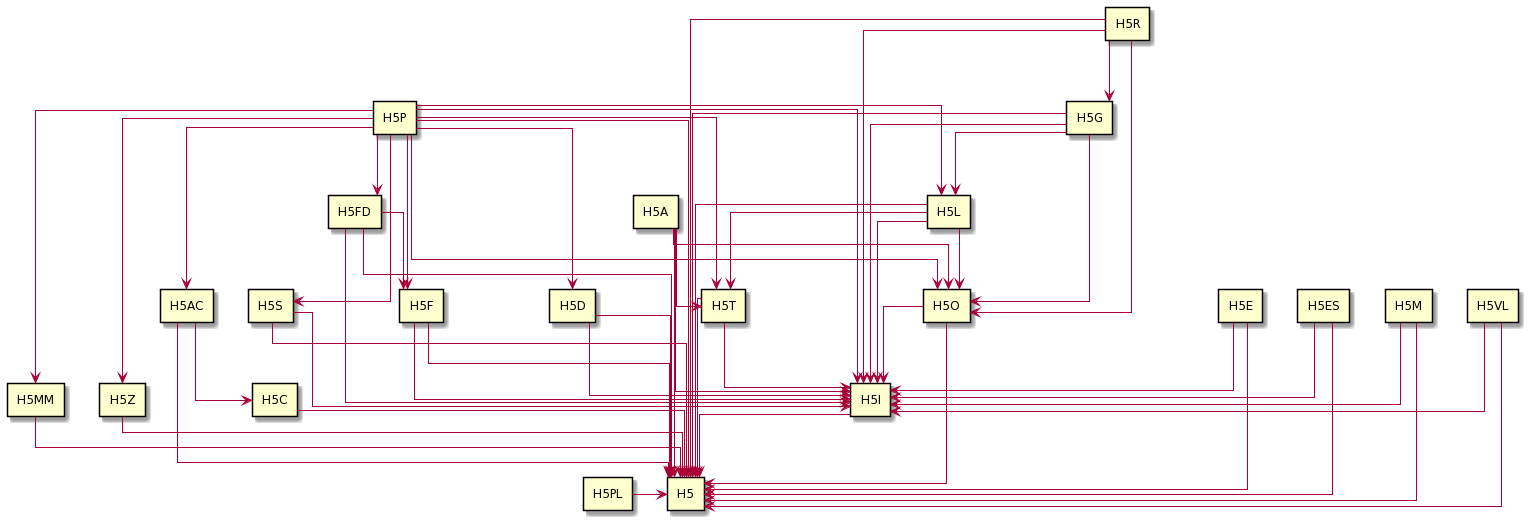
\includegraphics[scale=0.4,angle=90]{images/packackages-public-dependence.png}
\caption{The public dependence of HDF5 library modules as a directed graph.\label{fig:pub-module-dep}}
\end{sidewaysfigure}
\end{landscape}

% @startuml

% skin rose
% skinparam defaultFontSize 12
% skinparam backgroundColor transparent
% left to right direction

% rectangle "H5" {
%   rectangle public as h5public
% }
% package "H5A" {
%   rectangle public as h5apublic
%   rectangle private as h5aprivate
%   rectangle pkg as h5apkg
% }
% rectangle "H5B2" {
%   rectangle private as h5b2private
% }
% rectangle "H5FL" {
%   rectangle private as h5flprivate
% }
% rectangle "H5G" {
%   rectangle private as h5gprivate
% }
% rectangle "H5HF" {
%   rectangle private as h5hfprivate
% }
% rectangle "H5I" {
%   rectangle public as h5ipublic
% }
% rectangle "H5O" {
%   rectangle public as h5opublic
%   rectangle private as h5oprivate
% }
% rectangle "H5S" {
%   rectangle private as h5sprivate
% }
% rectangle "H5T" {
%   rectangle public as h5tpublic
%   rectangle private as h5tprivate
% }

% h5apublic --> h5public
% h5apublic --> h5ipublic
% h5apublic --> h5opublic
% h5apublic --> h5tpublic

% h5aprivate -[dashed]-> h5gprivate
% h5aprivate -[dashed]-> h5oprivate
% h5aprivate -[dashed]-> h5sprivate
% h5aprivate -[dashed]-> h5tprivate

% h5apkg -[dotted]-> h5b2private
% h5apkg -[dotted]-> h5flprivate
% h5apkg -[dotted]-> h5hfprivate
% h5apkg -[dotted]-> h5oprivate
% h5apkg -[dotted]-> h5sprivate
% h5apkg -[dotted]-> h5tprivate

% @enduml

\begin{figure}[!ht]
  \centering
  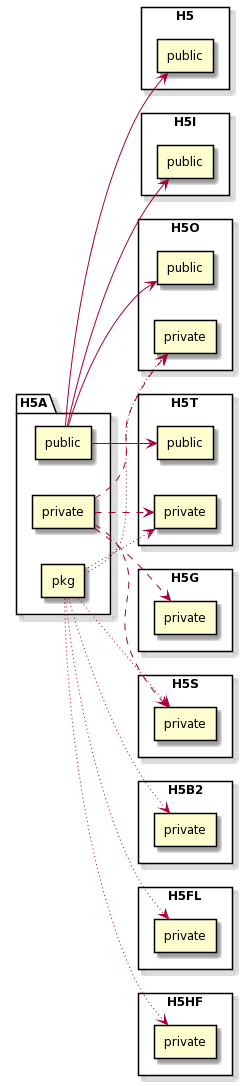
\includegraphics[scale=0.55]{images/H5A-dependence.png}
  \caption{\texttt{H5A} package dependence across visibilities.}
  \label{fig:h5a-dep}
\end{figure}

% \begin{table}
%   \centering
%  \caption{Internal package dependencies (in HDF5 1.14.3 - will change over time)}
% \label{table:mod-dep}
% {\tiny %
% \setlength\tabcolsep{2.25pt} % default value: 6pt
% \begin{tabular}{||c|c|c|c|c|c|c|c|c|c|c|c|c|c|c|c|c|c|c|c|c|c|c|c|c|c|c|c|c|c|c|c|c|c|c|c|c|c|c|c|c|c|c|c||}
% \hline
%   $\rightarrow$
%   & \texttt{A} & \texttt{AC} & \texttt{B} & \texttt{B2} & \texttt{C} & \texttt{CS} & \texttt{CX} & \texttt{D} & \texttt{E} &\texttt{EA}
%   & \texttt{ES} & \texttt{F} & \texttt{FA} & \texttt{FD} & \texttt{FL} & \texttt{FO} & \texttt{FS} & \texttt{G} & \texttt{H5} & \texttt{HF}
%   & \texttt{HG} & \texttt{HL} & \texttt{I} & \texttt{L} & \texttt{M} & \texttt{MF} & \texttt{MM} & \texttt{O} & \texttt{P} & \texttt{PB}
%   & \texttt{PL} & \texttt{R} & \texttt{RS} & \texttt{S} & \texttt{SL} & \texttt{SM} & \texttt{T} & \texttt{TS} & \texttt{UC} & \texttt{VL}
%   & \texttt{VM} & \texttt{WB} & \texttt{Z} \\ [0.5ex] 
% \hline\hline
% \texttt{A} & \textopenbullet & & & & & & \textbullet & & \textbullet & & \textbullet & & & & \textbullet & & & & \textbullet & & & & \textbullet & & & & \textbullet & \textbullet & & & & & & \textbullet & & & & & & \textbullet & & & \\ \hline
% \texttt{AC} & & \textopenbullet & & & \textbullet & & \textbullet & & \textbullet & & & \textbullet & & & & & & & \textbullet & & & & \textbullet & & & & \textbullet & & \textbullet & & & & & & \textbullet & & & & & & & & \\ \hline
% \texttt{B} & & & \textopenbullet & & & & \textbullet & & \textbullet & & & & & & & & & & \textbullet & & & & \textbullet & & & \textbullet & \textbullet & & \textbullet & & & & & & & & & & & & & & \\ \hline
% \texttt{B2} & & \textbullet & & \textopenbullet & & & & & \textbullet & & & \textbullet & & & \textbullet & & & \textopenbullet & \textbullet & & & & & & & \textbullet & \textbullet & & & & & & & & & & & & & & \textbullet & & \\ \hline
% \texttt{C} & & \textbullet & & & \textopenbullet & & \textbullet & & \textbullet & & & \textbullet & & \textbullet & \textbullet & & & & \textbullet & & & & & & & \textbullet & \textbullet & & & & & & & & & & & & & & \textbullet & & \\ \hline
% \texttt{CS} & & & & & & \textopenbullet & & & \textbullet & & & & & & & & & & \textbullet & & & & & & & & & & & & & & & & & & & & & & & & \\ \hline
% \texttt{CX} & & & & & & & \textopenbullet & \textbullet & \textbullet & & & & & & \textbullet & & & & \textbullet & & & & \textbullet & \textbullet & & & \textbullet & & \textbullet & & & & & & & & & & & & & & \\ \hline
% \texttt{D} & & \textbullet & \textbullet & & & & \textbullet & \textopenbullet & \textbullet & \textbullet & \textbullet & & \textbullet & \textbullet & \textbullet & \textbullet & & \textbullet & \textbullet & & \textbullet & \textbullet & \textbullet & \textbullet & & \textbullet & \textbullet & \textbullet & \textbullet & \textbullet & & & & \textbullet & & & & & & \textbullet & \textbullet & \textbullet & \\ \hline
% \texttt{E} & & & & & & & & & \textopenbullet & & & & & & \textbullet & & & & \textbullet & & & & \textbullet & & & & \textbullet &  & & & & & & & & & & \textbullet & & & & & \\ \hline
% \texttt{EA} & & & & & & & & & \textbullet & \textopenbullet & & & & & \textbullet & & & & \textbullet & & & & & & & \textbullet & \textbullet & & & & & & & & & & & & & & \textbullet & \textbullet & \\ \hline
% \texttt{ES} & & & & & & & & & \textbullet & & \textopenbullet & & & & \textbullet & & & & \textbullet & & & & & & & & \textbullet & & & & & & \textbullet & & & & & & & & & & \\ \hline
% \texttt{F} & & \textbullet & & & & & \textbullet & \textbullet & \textbullet & & \textbullet & \textopenbullet & & & \textbullet & \textbullet & & \textbullet & \textbullet & & \textbullet & & \textbullet & \textbullet & & \textbullet & \textbullet & \textbullet & \textbullet & \textbullet & & & & \textbullet & & \textbullet & \textbullet & & & \textbullet &  & & \\ \hline
% \texttt{FA} & & & & & & & & & \textbullet & & & & \textopenbullet & & \textbullet & & & & \textbullet & & & & & & & \textbullet & \textbullet & \textbullet & & & & & & & & & & & & & \textbullet & \textbullet & \\ \hline
% \texttt{FD} & & & & & & & \textbullet & \textbullet & \textbullet & & & \textbullet & & \textopenbullet & \textbullet & & & & \textbullet & & & & \textbullet & & & & \textbullet & & \textbullet & & \textbullet & & & & \textbullet & & & & & & & & \\ \hline
% \texttt{FL} & & & & & & \textbullet & & & \textbullet & & & & & & \textopenbullet & & & & \textbullet & & & & & & & & \textbullet &  & & & & & & & & & & & & & & & \\ \hline
% \texttt{FO} & & & & & & & & & \textbullet & & & \textbullet & & & \textbullet & \textopenbullet & & & \textbullet & & & & & & & & & \textbullet & & & & & & & & & & & & & & & \\ \hline
% \texttt{FS} & & \textbullet & & & & & & & \textbullet & & & \textbullet & & & & & \textopenbullet & & \textbullet & \textbullet & & & & & & \textbullet & \textbullet & & & & & & & & & & & & & & \textbullet & \textbullet & \\ \hline
% \texttt{G} & & \textbullet & & & & & \textbullet & \textbullet & \textbullet & & \textbullet & \textbullet & & & \textbullet & \textbullet & & \textopenbullet & \textbullet & & & \textbullet & \textbullet & \textbullet & & \textbullet & \textbullet & \textbullet & \textbullet & & & & & & \textbullet & & & & & \textbullet & & \textbullet & \\ \hline
% \texttt{H5} & & \textbullet & & & & & \textbullet & \textbullet & \textbullet & & & & & & \textbullet & & \textbullet & & \textopenbullet & & & & & \textbullet & & & \textbullet & & \textbullet & & \textbullet & & & & \textbullet & & \textbullet & & & & & & \\ \hline
% \texttt{HF} & & \textbullet & & \textbullet & & & & & \textbullet & & & \textbullet & & & \textbullet & \textbullet & & & \textbullet & \textopenbullet & & & & & & \textbullet & \textbullet & & & & & & & & & & & & & & \textbullet & \textbullet & \\ \hline
% \texttt{HG} & & \textbullet & & & & & & & \textbullet & & & \textbullet & & & & & & & \textbullet & & \textopenbullet & & \textbullet & & & \textbullet & \textbullet & & & & & & & & & & & & & & & & \\ \hline
% \texttt{HL} & & \textbullet & & & \textbullet & & & & \textbullet & & & \textbullet & & & \textbullet & & & & \textbullet & & & \textopenbullet & & & & \textbullet & \textbullet & & & & & & & & & & & & & & & & \\ \hline
% \texttt{I} & & & & & & & \textbullet & \textbullet & \textbullet & & & \textbullet & & & \textbullet & & & \textbullet & \textbullet & & & & \textopenbullet & & & & \textbullet & & \textbullet & & & & \textbullet & & & & \textbullet & & & \textbullet & & & \\ \hline
% \texttt{L} & & \textbullet & & & & & \textbullet & & \textbullet & & \textbullet & \textbullet & & & & & & \textbullet & \textbullet & & & & \textbullet & \textopenbullet & & & \textbullet & \textbullet & \textbullet & & & & & & & & & & & \textbullet & & & \\ \hline
% \texttt{M} & & & & & & & \textbullet & & \textbullet & & \textbullet & & & & & & & & \textbullet & & & & \textbullet & & \textopenbullet & & & & & & & & & & & & & & & \textbullet & & & \\ \hline
% \texttt{MF} & & & & & & & & & \textbullet & & & \textbullet & & & & & \textbullet & & \textbullet & & & & \textbullet & & & \textopenbullet & & & & & & & & & & & & & & & \textbullet & & \\ \hline
% \texttt{MM} & & & & & & & & & \textbullet & & & & & & & & & & \textbullet & & & & & & & & \textopenbullet & & & & & & & & & & & & & & & & \\ \hline
% \texttt{O} & \textbullet & \textbullet & & & & & \textbullet & \textbullet & \textbullet & & \textbullet & \textbullet & & & \textbullet & \textbullet & & \textbullet & \textbullet & \textbullet & \textbullet & \textbullet & \textbullet & \textbullet & & \textbullet & \textbullet & \textopenbullet & \textbullet & & & \textbullet & & \textbullet & & \textbullet & \textbullet & & & \textbullet & \textbullet & \textbullet & \textbullet \\ \hline
% \texttt{P} & & \textbullet & \textbullet & & & & \textbullet & \textbullet & \textbullet & & & \textbullet & & \textbullet & \textbullet & & & \textbullet & \textbullet & & & & \textbullet & \textbullet & \textbullet & & \textbullet & \textbullet & \textopenbullet & & & & & \textbullet & & & \textbullet & & & \textbullet & \textbullet & & \textbullet \\ \hline
% \texttt{PB} & & & & & & & & & \textbullet & & & \textbullet & & \textbullet & & & & & \textbullet & & & & \textbullet & & & & \textbullet & & & \textopenbullet & & & & & \textbullet & & & & & & & & \\ \hline
% \texttt{PL} & & & & & & & & & \textbullet & & & & & & & & & & \textbullet & & & & & & & & \textbullet & & & & \textopenbullet & & & & & & & & & & & & \textbullet \\ \hline
% \texttt{R} & & & & & & & \textbullet & & \textbullet & & & & & & & & & & \textbullet & & & & \textbullet & & & & \textbullet & & & & & \textopenbullet & & \textbullet & & & & & & \textbullet & & & \\ \hline
% \texttt{RS} & & & & & & & & & \textbullet & & & & & & \textbullet & & & & \textbullet & & & & & & & & & & & & & & \textopenbullet & & & & & & & & & & \\ \hline
% \texttt{S} & & & & & & & \textbullet & \textbullet & \textbullet & & & \textbullet & & & \textbullet & & & & \textbullet & & & & \textbullet & & & & \textbullet & \textbullet & & & & & & \textopenbullet & & & & & & & \textbullet & & \\ \hline
% \texttt{SL} & & & & & & & & & \textbullet & & & & & & \textbullet & & & & \textbullet & & & & & & & & \textbullet & & & & & & & & \textopenbullet & & & & & & & & \\ \hline
% \texttt{SM} & & \textbullet & & & & & & & \textbullet & & & \textbullet &  & & \textbullet & & & & \textbullet & & & & & & & \textbullet & \textbullet & \textbullet & & & & & & & & \textopenbullet & & & & & & \textbullet & \\ \hline
% \texttt{T} & & \textbullet & & & & & \textbullet & \textbullet & \textbullet & & \textbullet & \textbullet & & & \textbullet & \textbullet & & \textbullet & \textbullet & & & & \textbullet & \textbullet & & & \textbullet & \textbullet & \textbullet & & & \textbullet & & & & & \textopenbullet & & & \textbullet & & \textbullet & \\ \hline
% \texttt{TS} & & & & & & & & & \textbullet & & & & & & & & & & \textbullet & & & & & & & & \textbullet & & & & & & & & & & & \textopenbullet & & & & & \\ \hline
% \texttt{UC} & & & & & & & & & \textbullet & & & & & & \textbullet & & & & & & & & & & & & & & & & & & & & & & & & \textopenbullet & & & & \\ \hline
% \texttt{VL} & \textbullet & \textbullet & & & \textbullet & & \textbullet & \textbullet & \textbullet & & \textbullet & \textbullet & & & \textbullet & & & \textbullet & \textbullet & & \textbullet & & \textbullet & \textbullet & \textbullet & \textbullet & \textbullet & \textbullet & \textbullet & \textbullet & \textbullet & & & \textbullet & \textbullet & & \textbullet & & & \textopenbullet & & & \\ \hline
% \texttt{VM} & & & & & & & & & \textbullet & & & & & & & & & & \textbullet & & & & & & & & \textbullet & \textbullet & & & & & & & & & & & & & \textopenbullet & & \\ \hline
% \texttt{WB} & & & & & & & & & \textbullet & & & & & & \textbullet & & & & \textbullet & & & & & & & & & & & & & & & & & & & & & & & \textopenbullet & \\ \hline
% \texttt{Z} & & & & & & & \textbullet & \textbullet & \textbullet & & & \textbullet & & & & & & & \textbullet & & & & \textbullet & & & & \textbullet & \textbullet & \textbullet & & \textbullet & & & \textbullet & & & & & & & & & \textopenbullet \\
% \hline
% \end{tabular}
% }%
% \end{table}